\documentclass{article}

\usepackage{amsmath, graphicx}
\graphicspath{ {./images/} }

\title{Ch. 15 HW \#4 -- Solutions}
\author{Principles of Microeconomics}
\date{\today}

\begin{document}

\maketitle

\section*{Quick Quiz}

\begin{enumerate}

\setcounter{enumi}{5}
\item (d) -- Firms will produce the quantity at which $P = MC$ because they're profit maximizers. They'll enter or exit the market until profits are zero which happens when $P = ATC$.

\item (c) -- Firms will produce the quantity at which $P = MC$ because they're profit maximizers. If new firms want to enter, profits must be positive which means $P > ATC$.

\item (c) -- In the short run, the tax is an increase in fixed costs. Since MC and AVC don't shift, it doesn't change firm's short run quantity produced, so the number of pretzels consumed stays the same. In the long run, firms exit the market because ATC shifts up which makes profit negative. When firms exit, the quantity produced decreases, so the number of pretzels consumed decreases.

\end{enumerate}

\section*{Problems \& Applications}

\begin{enumerate}

\item 

	\begin{enumerate}
	
	\item An increase in the price of an input increases variable costs. As a result, marginal cost and average total cost shift up/left. The short run supply curve is the sum of all firms' marginal cost curves, so the short run supply curve shifts left as well. The long run supply curve is perfectly elastic at the price where firms make zero profit. Since that price increases when average total cost increases, the long run supply curve shifts up.
	
		\begin{center}
		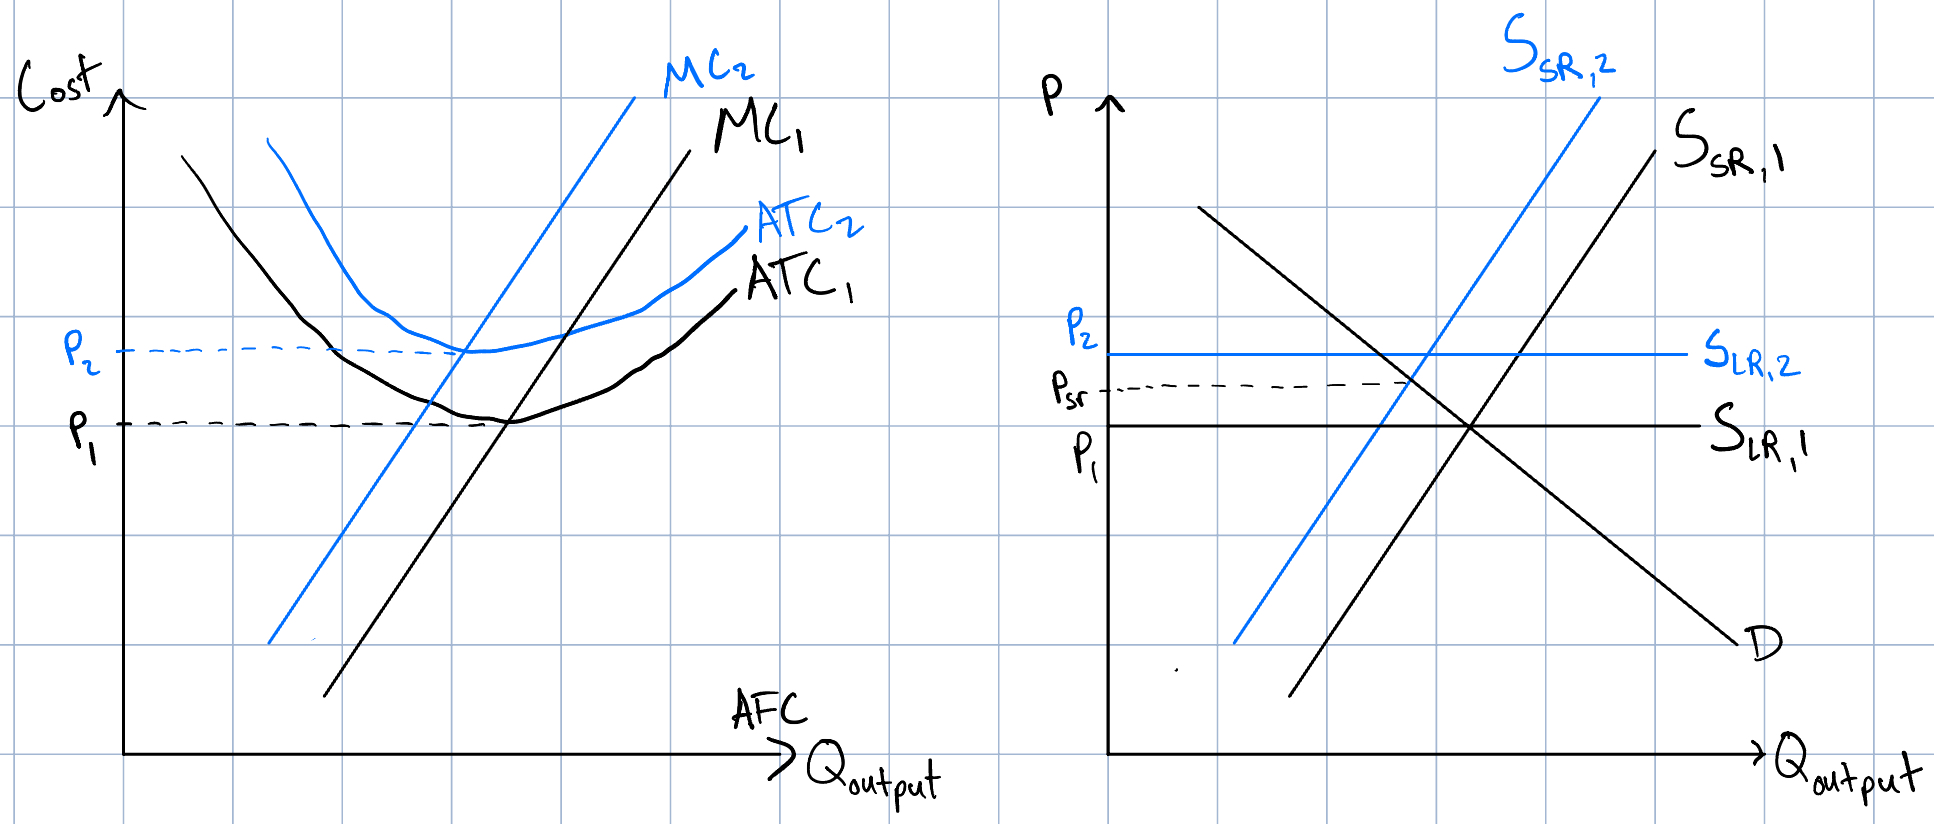
\includegraphics[width = \textwidth]{paa1a}
		\end{center}
		
	\item In the short run, profits depend on the elasticity of demand. As I drew it above, the short run price, $P_{SR}$, is below the new price at which firms make zero profit, $P_2$. In that case, profits become negative. If demand were more inelastic, $P_{SR}$ could be above the price at which firms make zero profit. In that case profits become positive. If profits become negative, the number of firms will decrease because some will exit the market. If profits become positive, the number of firms will increase because some will enter the market.
	
	\end{enumerate}

\setcounter{enumi}{2}
\item

	\begin{enumerate}
	
	\item The firm should produce 5 or 6 units.
	
		\begin{center}
		\begin{tabular}{c | c | c | c | c | c | c | c | c}
		\textbf{Quantity} & 0 & 1 & 2 & 3 & 4 & 5 & 6 & 7 \\
		\hline
		\textbf{Profit} & -8 & -1 & 6 & 13 & 19 & 21 & 21 & 19
		\end{tabular}
		\end{center}
		
	\item They intersect at a quantity of 5.5. That's consistent with my answer to (a). 
	
		\begin{center}
		\begin{tabular}{c | c | c | c | c | c | c | c | c}
		\textbf{Quantity} & 0 & 1 & 2 & 3 & 4 & 5 & 6 & 7 \\
		\hline
		\textbf{MR} & -- & 8 & 8 & 8 & 8 & 8 & 8 & 8 \\
		\hline
		\textbf{MC} & -- & 1 & 1 & 1 & 2 & 6 & 8 & 10
		\end{tabular}
		\end{center}
		
	\item It does look like the industry is competitive because marginal revenue is constant regardless of how much the firm produces. That implies that the firm is a price taker. The industry isn't in long run equilibrium because the firm has non-zero profit.
	
	\end{enumerate}
	
\setcounter{enumi}{4}
\item

	\begin{enumerate}
	
	\item I show the long run supply curve. In order to show the short run supply curve, you would have to add in the AVC curve.
	
		\begin{center}
		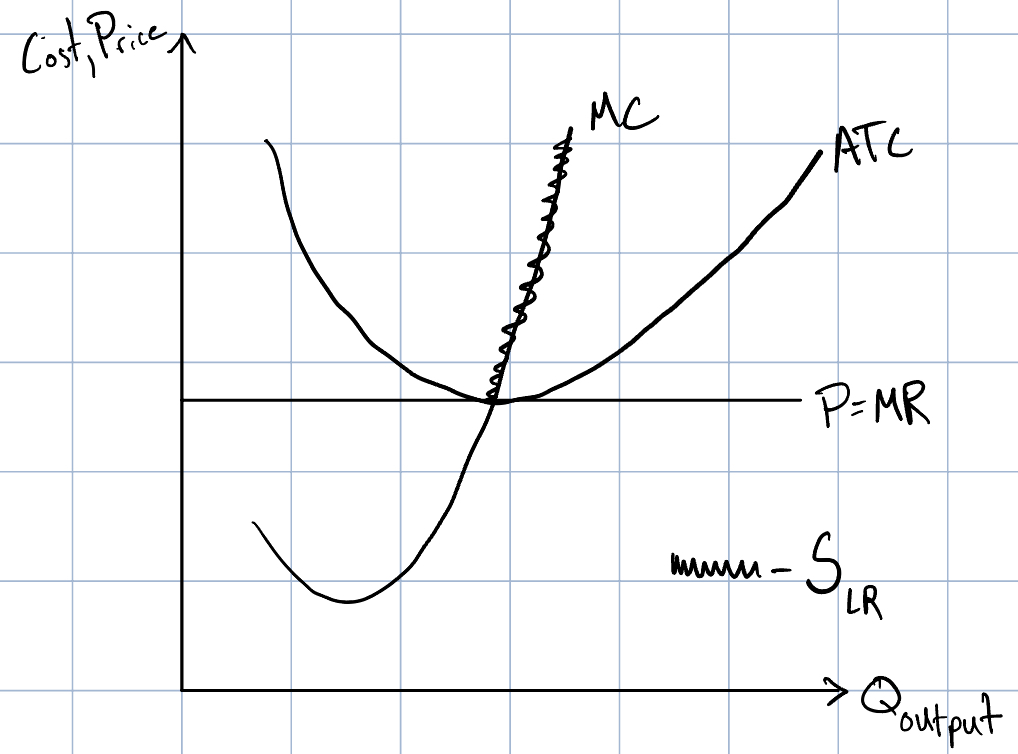
\includegraphics[width = 0.5\textwidth]{paa5a}
		\end{center}
		
	\item Hi-Tech's ATC curve shifts down, but all the other firms' ATC curves remain the same. Since it's a competitive market, Hi-Tech is a price taker, and the price of books remains the same. Profit is $(P - ATC)Q$, and $P - ATC$ increases, so Hi-Tech's profit increases.
	
	\item In the long run, when all the firms adopt the technology, all of their ATC curves shift down. Firms will enter or exit the market until price equals the minimum of the firms' ATC curves and profits equal zero. 
	
	\end{enumerate}
	
\setcounter{enumi}{7}
\item

	\begin{enumerate}
	
	\item Price is equal to marginal cost, greater than average variable cost, and less than average total cost. 
	
	\item \phantom{x}
	
		\begin{center}
		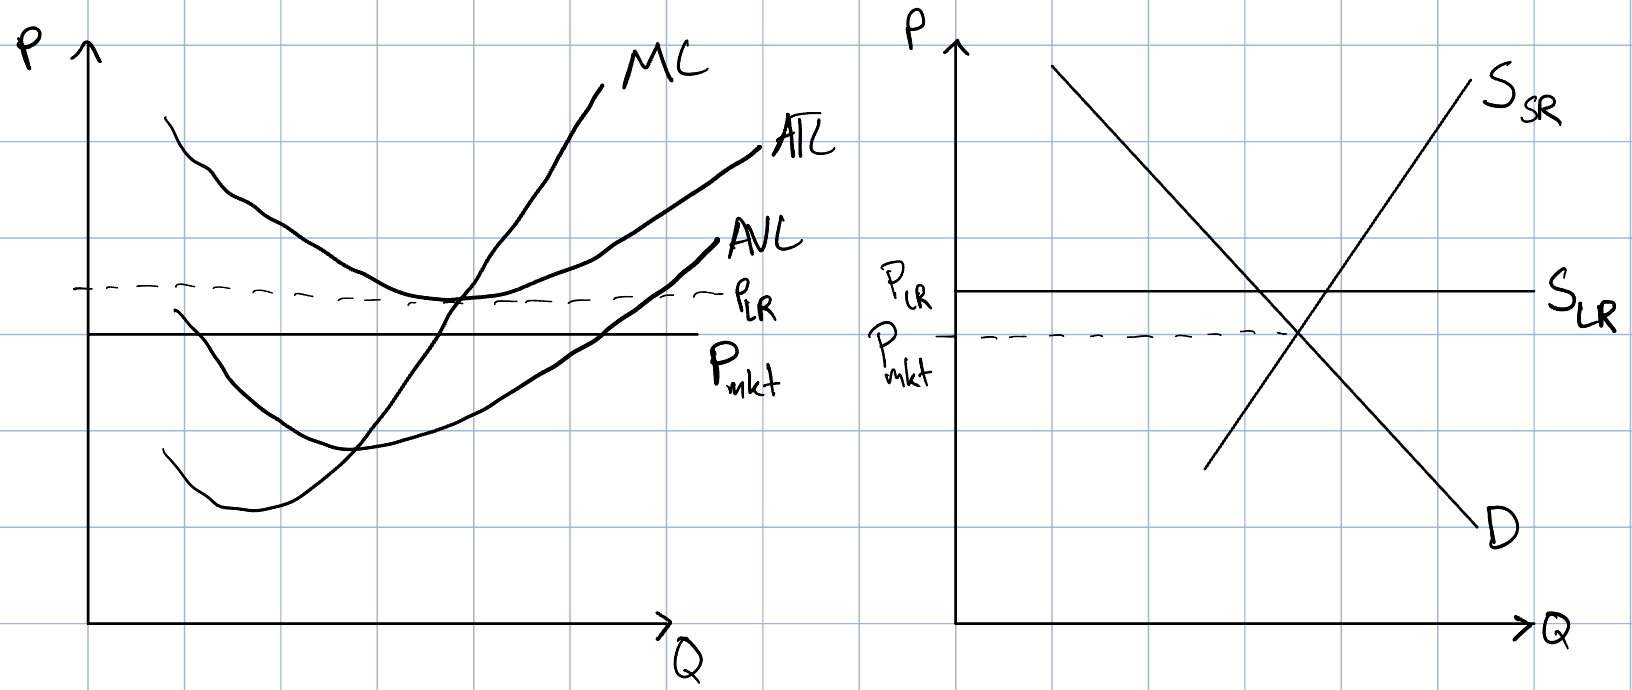
\includegraphics[width = \textwidth]{paa8b}
		\end{center}
		
	\item Firms leave the market because they are making losses. That decreases the number of suppliers which shifts short-run market supply left. When short-run market supply shifts left, price increases until profits are zero, and total quantity supplied decreases. The marginal cost and average total cost curves remain the same, so when price increases, firms start producing more. That means the quantity supplied by each firm still in the market increases.
	
	\end{enumerate}

\end{enumerate}

\end{document}